\section{Method}\label{method}

\subsection{System Overview \& Problem
    Formulation}\label{system-overview--problem-formulation}

\begin{figure*}
    \centering
    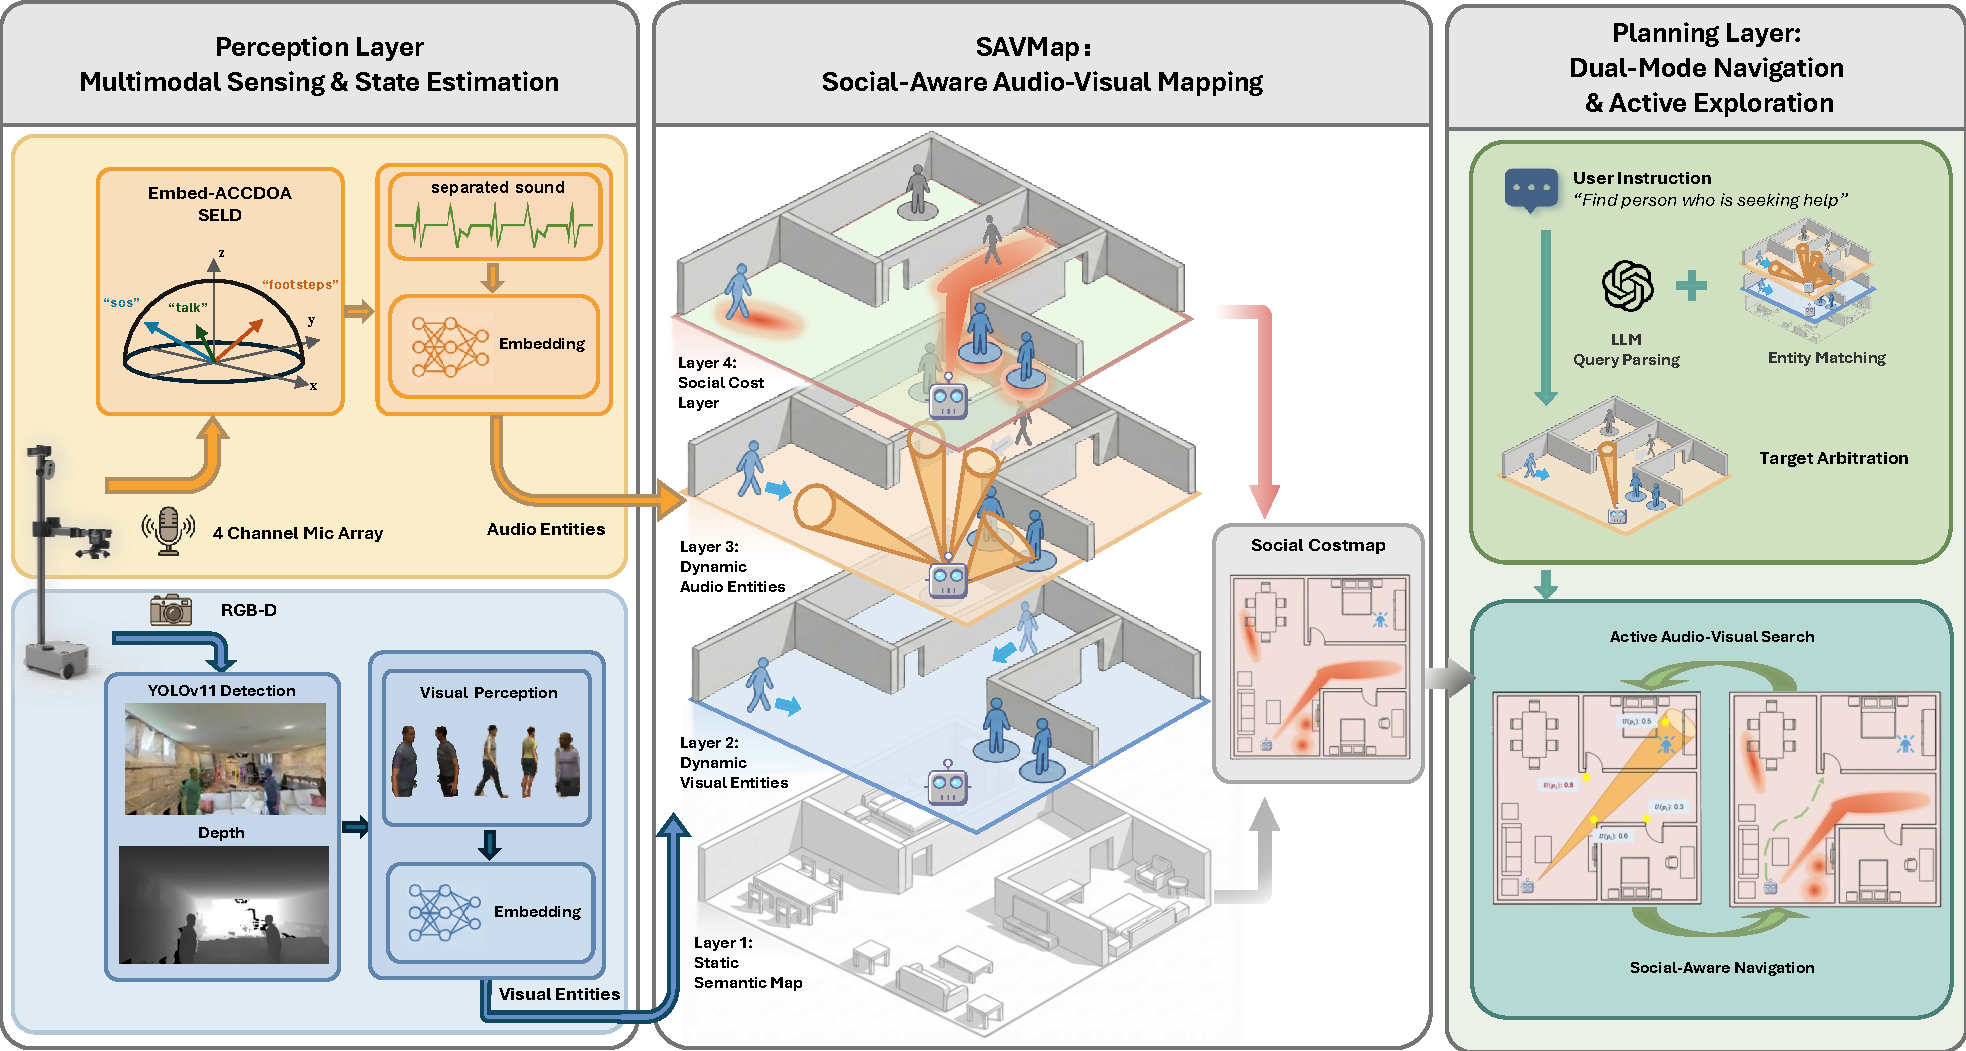
\includegraphics[width=1\linewidth]{figures/method}
    \caption{\textbf{Overview of the SAVNav pipeline.}
    In the Perception Layer, an RGB-D camera performs human detection and 3D localization, while a 4-channel microphone array runs Sound Event Localization and Detection (SELD) to estimate Direction-of-Arrival (DoA) and semantic labels, forming \textit{visual/audio entities} with spatial and semantic attributes. SAVMap (Social-Aware Audio-Visual Mapping) fuses these observations into a layered grid representation: Layer 1 Static Semantic Map, Layer 2 Dynamic Visual Entities, Layer 3 Dynamic Audio Entities, and Layer 4 Social Cost Layer, producing a \textit{Social Costmap} for planning. In the Planning Layer, an MLLM parses the user instruction for query parsing and entity matching to select the best-matching target, and then switches between \textit{Social-Aware Navigation} and \textit{Active Audio-Visual Search} (Search--Then--Go) to disambiguate audio-only cues and mitigate Non-Line-of-Sight (NLOS) risks.}
    
    \label{fig:savnav-method}
\end{figure*}

We consider a mobile robot operating in a dynamic, semi-structured
indoor environment populated by human agents. The robot is equipped with
an RGB-D camera and a 4-channel microphone array.

Coordinate Systems: We define the World Frame \(\mathcal{W}\) with the
origin at the scene center and the Ego Frame \(\mathcal{E}\) attached to
the robot\textquotesingle s geometric center. Let
\(\mathbf{x}_t = [x, y, z, \psi]^T\) denote the robot\textquotesingle s
pose in \(\mathcal{W}\) at time \(t\).

Problem Definition: Given a natural language instruction \(\mathcal{I}\)
(e.g., \emph{"Find the person talking"}), the objective is to generate a
sequence of control actions \(a_{t} \in \mathcal{A}\) to navigate
towards the target location \(\mathbf{g}^*\) while minimizing the
traversal time and ensuring social compliance. This requires handling
two types of entities: Observable Entities (within the
camera\textquotesingle s Field-of-View, FoV) and Occluded Acoustic
Sources (Non-Line-of-Sight, NLOS).

\subsection{Multi-Modal Perception with
    Uncertainty}\label{multi-modal-perception-with-uncertainty}

Our perception stack processes visual and auditory streams
asynchronously to extract semantic and spatial information, explicitly
modeling the uncertainty inherent in each modality.

\subsubsection{Visual Perception}\label{visual-perception}

The visual module runs at camera frame rate (\(\sim\) 20Hz). We employ
YOLOv11 \cite{YOLOv11OverviewKey2024} for 2D object detection and
segmentation. For each detected bounding box, we compute the 3D centroid
\(\mathbf{p}_{vis}^{\mathcal{E}}\) in the Ego Frame using depth data.
To account for sensor noise and partial occlusions, we model the
positional uncertainty \(\sigma_{p}\) as:

\begin{equation}
    \sigma_{p} = k_d \cdot z^2 + k_{occ} \cdot \left(1 - \frac{N_{mask}}{N_{box}}\right)
    \label{eq:positional-uncertainty}
\end{equation}
where \(z\) is the depth, \(k_d\) captures the depth
sensor\textquotesingle s quadratic error characteristics, and the second
term penalizes occlusion based on the mask-to-box ratio with coefficient
\(k_{occ}\). We extract semantic features \(\mathbf{f}_{vis}\) using
ImageBind \cite{ImageBindOneEmbedding2023} and appearance features
\(\mathbf{f}_{reid}\) for temporal tracking.

\subsubsection{Audio Perception}\label{audio-perception}

The audio module processes 4-channel ambisonic signals in a sliding
window (2.55s duration, 0.5s stride), ensuring a system latency of \(\sim\)0.5s despite the long temporal context. We utilize Embed-ACCDOA
\cite{OpenvocabularySoundEvent2025} for Sound Event Localization and
Detection (SELD).
For each frame, the model predicts the Direction-of-Arrival (DoA) vector
\(\mathbf{v}_{doa} \in \mathbb{R}^3\) and a semantic label. The angular
uncertainty \(\sigma_{ang}\) is dynamically scaled by the detection
confidence \(c\):

\begin{equation}
    \sigma_{ang} = \sigma_{base} \cdot (1 + k_{unc} \cdot (1 - c))
    \label{eq:angular-uncertainty}
\end{equation}
where \(\sigma_{base}\) is the empirical error margin of the SELD model.
Unlike vision, audio lacks direct distance information; thus, we model
the source position as a probability cone
\(\mathcal{C}_{audio}(\mathbf{x}_t, \mathbf{v}_{doa}, \sigma_{ang})\)
originating from the robot.

\subsection{SAVMap: Spatio-Temporal
    Mapping}\label{savmap-spatio-temporal-mapping}

We introduce SAVMap, a layered grid map (0.05m resolution) that
integrates static semantics with dynamic audio-visual entities to
support socially-aware navigation.

\subsubsection{Entity Tracking and
    Association}\label{entity-tracking-and-association}

We maintain a list of tracked entities using Kalman filtering for position estimation and Exponential Moving Average (EMA) for feature smoothing. For visual observations, we
employ a Hungarian matching algorithm based on a hybrid cost matrix
\(C_{ij}\):

\begin{equation}
    C_{ij} = w_{pos} \cdot \|\mathbf{p}_i - \mathbf{p}_j\| + w_{emb} \cdot (1 - \cos(\mathbf{f}_i, \mathbf{f}_j))
    \label{eq:hungarian-cost}
\end{equation}

For audio observations, we perform cross-modal association. If an audio
source DoA aligns with a visual entity within \(\sigma_{ang}\) and shares semantic consistency
(e.g., "speech" vs. "person"), it is \textit{anchored} to the visual target.
To ensure robustness against occlusion, we employ a \textbf{De-anchoring} mechanism: if an anchored visual entity exits the FoV for a duration \(T_{break}\) (e.g., 2.0s) while the audio signal persists, the entity reverts to an unanchored state, triggering the fallback momentum injection logic.

\subsubsection{Topology-Aware Acoustic Hallucinated
    Momentum}\label{topology-aware-hallucinated-momentum}

A key contribution of our work is handling unanchored audio sources
(i.e., heard but not seen). To anticipate NLOS risks (e.g., a person
approaching from around a corner), we propose an \textit{Acoustic Hallucinated Momentum}
Injection mechanism:

\begin{enumerate}
    \def\labelenumi{\arabic{enumi}.}
    \item
          Ray-Casting: We project a ray along the unanchored DoA until it
          intersects with the static map boundaries.
    \item
          Topological Adsorption: The intersection point is snapped to the
          nearest topological node (e.g., a doorway or corner), denoted as the
          hallucinated position \(\mathbf{p}_{hall}\).
    \item
          Virtual Velocity: We assign a virtual velocity vector
          \(\mathbf{v}_{virt}\) to this entity, pointing directly towards the
          robot, simulating a worst-case collision scenario.
\end{enumerate}

\subsubsection{Social Cost Layer}\label{social-cost-layer}

We construct a unified cost map \(M_{cost}\) to guide the planner.

\begin{enumerate}
    \def\labelenumi{\arabic{enumi}.}
    \item
          Visible Humans: For tracked visual entities, we generate a Gaussian
          cost field. If the human is moving, the Gaussian is anisotropic,
          elongated along their velocity vector.
    \item
          Hallucinated Moving Sources: For unanchored sources with dynamic signatures (e.g., footsteps), we generate an Anisotropic Risk Field (``Lance-shaped'') aligned with \(\mathbf{v}_{virt}\) to implement ``Hearing before Seeing'':
          \begin{equation}
              J_{move}(\mathbf{x}) = A \cdot \mathbb{I}(d_{long} > 0) \cdot \exp \left( - \left( \frac{d_{long}^2}{2\sigma_{front}^2} + \frac{d_{lat}^2}{2\sigma_{lat}^2} \right) \right)
              \label{eq:audio-risk-move}
          \end{equation}
          where \(d_{long}, d_{lat}\) are longitudinal and lateral distances in the virtual velocity frame in the virtual velocity frame. This encourages wide turns around corners.
    \item
          Stationary Audio Sources: For static sources (e.g., speech), we employ a Dynamic Probabilistic Cone Field that decays with distance:
          \begin{equation}
              J_{stat}(\mathbf{x}) = \frac{A}{1 + \gamma \|\mathbf{x} - \mathbf{p}_{src}\|} \cdot \exp\left(-\frac{\theta_{dev}^2}{2\sigma_{ap}^2}\right)
              \label{eq:audio-risk-stat}
          \end{equation}
          where \(\theta_{dev}\) is the angular deviation from the DoA and \(\sigma_{ap}\) represents the aperture uncertainty.
    \item
          Target Immunity: To prevent the robot from being repelled by its goal, costs generated by the designated target entity are masked to zero.
\end{enumerate}

\subsection{SAVNav: Socially-Aware
    Planning}\label{savnav-socially-aware-planning}

To handle the ambiguity of audio data, we design a simple closed-loop
planner that alternates between goal-directed navigation (when the
target is visually anchored) and belief-driven active search (when the
target is audio-only and unanchored).

\subsubsection{Planning Loop (Search--Then--Go)}\label{sec:planning-loop}

The planner maintains a binary flag \(\texttt{target\_anchored}\). When
the target is visually confirmed and anchored, the robot navigates
towards the anchored goal using risk-aware global planning. Otherwise,
it actively selects informative viewpoints to reduce uncertainty until
the target becomes visually confirmed.

\subsubsection{Risk-Aware Path
    Generation (Go-to)}\label{sec:risk-aware-path-generation}

In this state, the goal \(\mathbf{g}^*\) is deterministic. We employ the
Fast Marching Method (FMM) to solve the Eikonal equation over the speed
field \(S(\mathbf{x}) = S_{max} \cdot (1 - M_{cost}(\mathbf{x})) + S_{min}\). We include a minimal speed term \(S_{min}\) to ensure mathematical reachability even in high-cost regions. The
gradient descent on the resulting arrival time map \(T(\mathbf{x})\)
yields a smooth, global path that naturally skirts high-social-cost
regions.

\subsubsection{Belief-Driven Active Search (Search)}\label{sec:belief-driven-active-search}

When the target is unanchored (audio-only), the robot switches to an active search mode to maximize the Probability of Detection (PoD). We maintain a grid-based Target Belief Map \(\mathcal{M}_{belief}\) initialized with a uniform prior.

\begin{algorithm}[t]
    \caption{Belief-Driven Active Search (Search--Then--Go)}
    \label{alg:active-search}
    \begin{algorithmic}[1]
        \REQUIRE Cost map \(M_{cost}\); belief map \(\mathcal{M}_{belief}\); audio DoA \(\mathbf{v}_{doa}\) (with \(\sigma_{ang}\)); candidate viewpoints \(\mathcal{P}\)
        \STATE Initialize \(\texttt{target\_anchored} \leftarrow \text{false}\)
        \WHILE{task not finished}
            \STATE Update \(\mathcal{M}_{belief}\) with audio evidence in \(\Omega_{ROI}\)
            \STATE Apply negative visual update in \(\text{FOV}_{free}\) (no target observed)
            \IF{consistent visual detection exists}
                \STATE Anchor target; set \(\texttt{target\_anchored} \leftarrow \text{true}\)
            \ENDIF
            \IF{\(\texttt{target\_anchored}\)}
                \STATE Plan to goal using FMM on \(M_{cost}\); execute
            \ELSE
                \FOR{each \(\mathbf{p} \in \mathcal{P}\)}
                    \STATE Compute utility \(U(\mathbf{p})\) (Eq.~\ref{eq:nbv-utility})
                \ENDFOR
                \STATE Select \(\mathbf{p}^* \leftarrow \arg\max_{\mathbf{p} \in \mathcal{P}} U(\mathbf{p})\)
                \STATE Plan to \(\mathbf{p}^*\) using FMM on \(M_{cost}\); execute
            \ENDIF
        \ENDWHILE
    \end{algorithmic}
\end{algorithm}

\paragraph{Belief Dynamics} The belief map is updated recursively based on audio-visual observations. Positive audio detections inject probability mass into the uncertainty cone \(\Omega_{ROI}\). Crucially, negative visual observations (seeing empty space) reduce belief in the observed region:
\begin{equation}
    \mathcal{M}_{t}(c) = \begin{cases}
        \text{clip}(\mathcal{M}_{t-1}(c) + \alpha \cdot G(c), 0, 1) & \text{Audio Update} \\
        \mathcal{M}_{t-1}(c) \cdot \lambda_{neg} & \text{Visual Negative}
    \end{cases}
\end{equation}
where \(\lambda_{neg} < 1\) is a forgetting factor for regions within \(\text{FOV}_{free}\).

\paragraph{Utility Maximization} We generate a diverse set of candidate viewpoints \(\mathcal{P}\) using GVD nodes, ROI-guided sampling, and in-situ reorientation. The Next-Best-View (NBV) is selected by maximizing an information-theoretic utility function:
\begin{equation}
    U(\mathbf{p}) = \underbrace{\sum_{c \in \text{FOV}(\mathbf{p})} [\mathcal{M}_{t}(c) \cdot \gamma(\|c-\mathbf{p}\|)]}_{\mathcal{I}_{gain}} - \beta \cdot \mathcal{C}_{travel}(\mathbf{p})
    \label{eq:nbv-utility}
\end{equation}
where \(\gamma(d)\) is a resolution decay factor that penalizes distant observations to ensure reliable detection. \(\mathcal{C}_{travel}\) represents the geodesic cost to the candidate pose. Upon visual confirmation, the specific entity is anchored and the planner proceeds with goal-directed navigation.

\subsubsection{Reactive Control}\label{reactive-control}

The planned path is executed by a local controller. To ensure safety, an
Emergency Brake is triggered if the Time-To-Collision (TTC) with any
dynamic obstacle (visual or hallucinated) drops below 1.0s.
